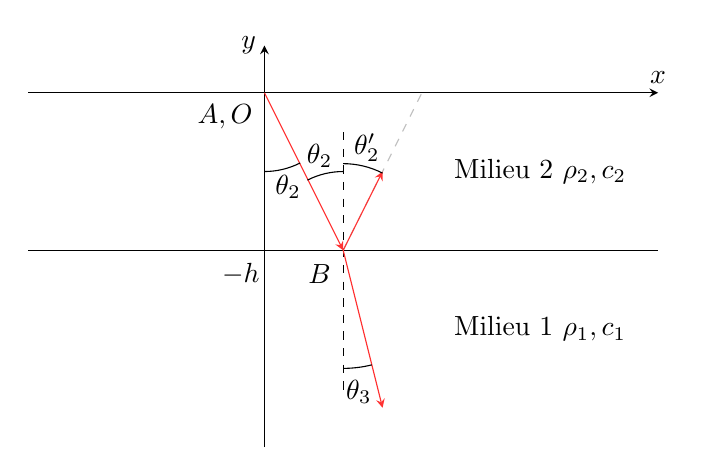
\begin{tikzpicture}

    % ifaces
    \draw [>=stealth, ->] (-3,0) -- (5,0);
    \draw (-3,-2) -- (5,-2);

    % Labels
    \draw (3.5,-1) node {Milieu 2 $\rho_2,c_2$};
    \draw (3.5,-3) node {Milieu 1 $\rho_1,c_1$};

    % verticals
    \draw [dashed] (0,.5) -- (0,-1.5);
    \draw [dashed] (1,-0.5) -- (1,-3.8);

    % axis
    %% y
    \draw [>=stealth, ->] (0,-4.5) -- (0,.6);
    \draw (-.2,.6) node {$y$};
    %% x (already drawn)
    \draw (5,.2) node {$x$};
    %% ordonnée h
    \draw (-.3,-2.3) node {$-h$};


    % points A & B
    \draw (-.5, -.3) node {$A,O$};
    \draw (.7, -2.3) node {$B$};

    % rays
    \draw [red!80, >=stealth, ->] (0,0) -- (1, -2);
    \draw [gray!50, dashed] (1,-2) -- (2,0);
    \draw [red!80, >=stealth, ->] (1,-2) -- (1.5, -1);
    \draw [red!80, >=stealth, ->] (1,-2) -- (1.5, -4);

    % angles
    \draw (0,-1) arc (-90:-63:1) node at (0.3,-1.2) {$\theta_2$};
    \draw (1,-1) arc (90:117:1) node at (.7,-.8) {$\theta_2$};
    \draw (1,-0.9) arc (90:63:1.1) node at (1.3,-.7) {$\theta_2'$};
    \draw (1,-3.5) arc (-90:-76:1.5) node at (1.2,-3.8) {$\theta_3$};


\end{tikzpicture}
